\section{Photon emission and absorption}
We have considered these processes before in section 5.2
\begin{dgroup}[]
	\begin{dmath}[]
		H=H_0+H_{\text{em}}+\hat{V}
		=\sum_{i}^{}\frac{p_{i}^{2}}{2m}+\frac{1}{8\pi}\int_{}^{}\rd^3 r \, \left( \hat{\vtr{E}}^2+\hat{\vtr{B}}^2 \right)+\text{interaction matter $\leftrightarrow$ photons}
	\end{dmath}
	\begin{dmath}[]
		\text{eigenstates }\ket{\psi_{\alpha}^{0}}=\ket{\text{matter}}\otimes \ket{\text{photons}}
		=\text{wave function}\otimes \text{new, Fockspace}
		=\ket{A;n_1\left( k,\lambda_1 \right)\ldots n_m\left( k_m,\lambda_m \right)}
	\end{dmath}
\end{dgroup}
\subsection{Absorption of photon}
\begin{dgroup}[]
	\begin{dmath}[]
		V_{\beta\alpha}=\mel{B;\left( n-1 \right)\left( k,\lambda \right)}{\hat{V}}{A;n\left( k,\lambda \right)}
	\end{dmath}
	\begin{dsuspend}
		with
		\begin{description}
			\item[$B$:] final state of atom
			\item[$\left( n-1 \right)$:] one photon ``lost''
			\item[$A$:]  initial state of atom
			\item[$n\left( k,\lambda \right)$:] $n$ photons, $k$, $\lambda$
		\end{description}
	\end{dsuspend}
	\begin{dmath}[]
		\hiderel{\leadsto} V_{\beta\alpha}=\frac{e}{mc}\int_{}^{}\frac{\rd^3 \vtr{k}}{\left( 2\pi \right)^3}\sum_{\lambda'}^{}\sqrt{\frac{2\pi \hbar c^2}{\omega'}}\cdot \mel{B;\left( n-1 \right)\left( k,\lambda \right)}{\hat{a}\left( k',\lambda' \right)\vtr{p}\cdot \vtr{\upepsilon}\left( k',\lambda' \right)e^{i\vtr{k}'\cdot \vtr{r}}}{A,n\left( k,\lambda \right)}	
	\end{dmath}
	\begin{dsuspend}
		$\hat{a}^{\dagger}$ term gives no contribution
	\end{dsuspend}
	\begin{dmath}[]
		\hiderel{\leadsto} V_{\beta\alpha}
		=\frac{e}{m}\sqrt{\frac{2\pi \hbar}{\omega}}\sqrt{n}\mel{B;}{\vtr{p}\cdot \vtr{\upepsilon}(k,\lambda)e^{i\vtr{k}\cdot \vtr{r}}}{A}\sim \sqrt{n}
	\end{dmath}
\end{dgroup}
\subsection{Emission of photons}
\begin{dgroup}[]
	\begin{dmath}[]
		V_{\beta\alpha}=\mel{B;\left( n+1 \right)\left( k,\lambda \right)}{\hat{V}}{A;n\left( k,\lambda \right)}
	\end{dmath},
	\begin{dsuspend}
		with $\hat{V}$ now anly $\hat{a}^{\dagger}$ part contribution.
	\end{dsuspend}
	\begin{dmath}[]
		\hiderel{\leadsto} V_{\beta\alpha} 
		=\frac{e}{m}\sqrt{\frac{2\pi\hbar}{\omega}}\sqrt{n+1}\mel{B}{\vtr{p}\cdot \vtr{\upepsilon}^{*}\left( k,\lambda \right)e^{-i\vtr{k}\cdot \vtr{r}}}{A}\sim \sqrt{n+1}
	\end{dmath}
\end{dgroup}
Note: This is non-zero even for $n=0$ $\to$ spontaneous emission!

recall classical:

\begin{dgroup}[]
	\begin{dmath}[]
		\Gamma_{n0}=\Gamma_{0n}
	\end{dmath}
	\begin{dmath}[]
		\text{absorption}=\text{emission}
	\end{dmath}
	\begin{dsuspend}
		now
	\end{dsuspend}
	\begin{dmath}[]
		\frac{\Gamma_{n0}}{\Gamma_{0n}}=\frac{n_{k\lambda}}{n_{k\lambda}+1}
	\end{dmath}
\end{dgroup}
\section{Scattering of photons by atoms}
\begin{figure}[]
	\begin{center}
		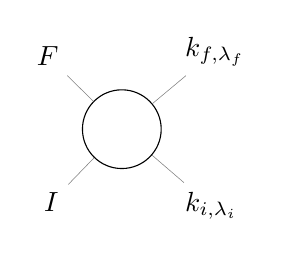
\begin{tikzpicture}[decoration=zigzag]
			\node[circle,draw,minimum size=1cm,pin=above left:$\ket{\vtr{F}}$,pin=below left:$\ket{I}$] (o) at (0,0) {};
			\begin{scope}[]
				\node[circle,minimum size=1cm,pin=above right:$\vtr{k}_{f,\lambda_{f}}$] (o2) at (0,0) {};
				\node[circle,minimum size=1cm,pin=below right:$\vtr{k}_{i,\lambda_{i}}$] (o2) at (0,0) {};
			\end{scope}
		\end{tikzpicture}
	\end{center}
	\caption{}
	\label{fig:}
\end{figure}
involves creation and annihilation of photon need $\hat{a}^{\dagger}\left( k_f,\lambda_f \right)\hat{a}\left( k_i,\lambda_i \right)$ recall
\begin{dmath}[]
	\hat{V}=\frac{e}{mc}\vtr{p}\cdot \hat{\vtr{A}}+\frac{e^{2}}{2mc^2}\hat{\vtr{A}}^2
\end{dmath}
where $\hat{\vtr{A}}$ contains either $\hat{a}^{\dagger}$ or $\hat{a}$ and cotributes only at 2nd order, $\hat{\vtr{A}}^2$ contains $\hat{a}^{\dagger}\hat{a}$ $\to$ contributes at first order. Both $\hat{\vtr{A}}$ and $\hat{\vtr{A}}^2$ are $\sim \frac{e^2}{c^2}$
\paragraph{first-order contribution}
\begin{dmath}[]
	V_{\beta\alpha}^{(1)}
	=\mel{F,1\left( k_f,\lambda_f \right)}{\frac{e^2}{2mc^2}\hat{\vtr{A}}^2}{I,1\left( k_i,f_i \right)}
	=\frac{e^2}{2mc^2}\int_{}^{}\frac{\rd^3 \vtr{k}}{(2\pi)^3}\int_{}^{}\frac{\rd^3 \vtr{k}'}{\left( 2\pi \right)^3}\sum_{\lambda\lambda'}^{}\frac{2\pi\hbar c^2}{\sqrt{\omega\omega'}}\cdot \bra{F,1\left( k_{f},\lambda_{f} \right)}\left( \hat{a}\vtr{\upepsilon}e^{i\vtr{k}\cdot \vtr{r}-i\omega t}+\hat{a}^{\dagger}\left( k,\lambda \right)e^{-i\vtr{k}\cdot \vtr{r}+i\omega t} \right)
	\cdot \left( \hat{a}'\left( k',\lambda' \right) e^{i\vtr{k}\cdot \vtr{r}-i\omega t}+\mbox{$\hat{a}^{\dagger}$}'{\vtr{\upepsilon}'}^{*}e^{-i\vtr{k}\cdot \vtr{r}+i'w t} \right)
\ket{ I,1\left( k_i,\lambda_i \right)}
=\frac{e^2}{2mc^2}\frac{2\pi \hbar c^2}{\sqrt{\omega_i\omega_f}}2\cdot
\mel{F}{\vtr{\upepsilon}\left( k_i,\lambda_i\cdot \vtr{\upepsilon}\left( k_f,\lambda_f \right)e^{it\left( \omega_i-\omega_f \right)} \right)e^{i\vtr{r}\cdot \left( \vtr{k}_i-\vtr{k}_f \right)}}{I}
\end{dmath}
